\begin{figure}[thbp]
\vspace{-0.5 cm}
\setlength{\abovecaptionskip}{.3 cm}
\setlength{\belowcaptionskip}{-.1 cm} 
	\centering
    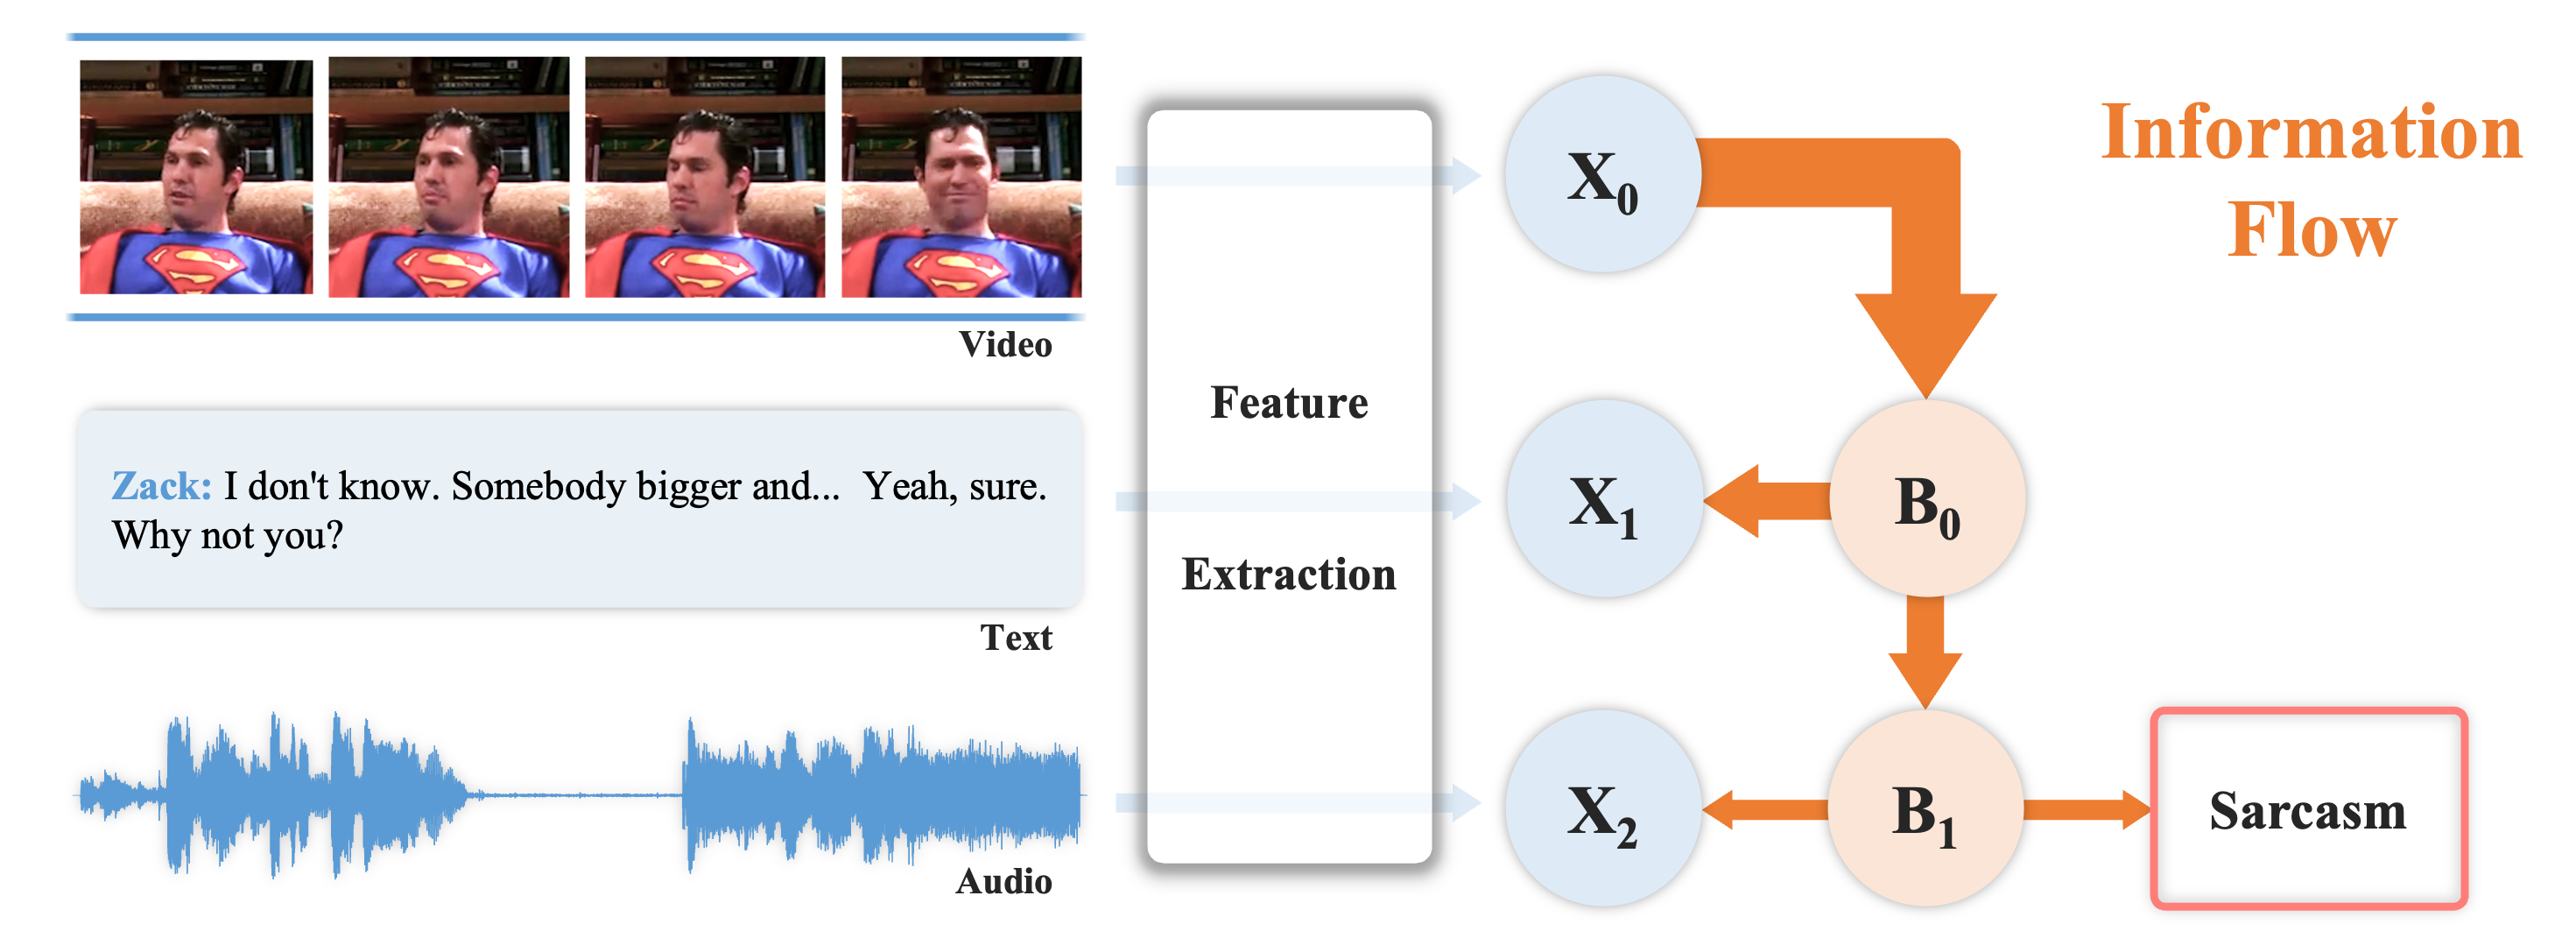
\includegraphics[width=.9\linewidth]{Figures/sarcasmDetection.png}
    \caption{\textbf{A schematic representation of our proposed ITHP and its information flow.} The diagram illustrates the process of feature extraction from multimodal embedding data including video frames, text, and audio patterns. These modalities pass through a ``Feature Extraction'' phase, where they are embedded to get modal states $X_0$, $X_1$, and $X_2$. The derived states are then processed to construct latent states $B_0$ and $B_1$. This processing includes reciprocal information exchange between $X_1$ and $B_0$, as well as between $B_1$ and $X_2$. The resulting information from this process is then used to make a determination about the presence of sarcasm.}
    \label{fig:sarcasmDetection}
\end{figure}